% --------------------------------------------------------------------------- %
% Poster for the ECCS 2011 Conference about Elementary Dynamic Networks.      %
% --------------------------------------------------------------------------- %
% Created with Brian Amberg's LaTeX Poster Template. Please refer for the     %
% attached README.md file for the details how to compile with `pdflatex`.     %
% --------------------------------------------------------------------------- %
% $LastChangedDate:: 2011-09-11 10:57:12 +0200 (V, 11 szept. 2011)          $ %
% $LastChangedRevision:: 128                                                $ %
% $LastChangedBy:: rlegendi                                                 $ %
% $Id:: poster.tex 128 2011-09-11 08:57:12Z rlegendi                        $ %
% --------------------------------------------------------------------------- %
\documentclass[a0paper,portrait]{baposter}

\usepackage[ngerman]{babel}
\usepackage{relsize}		% For \smaller
\usepackage{url}			% For \url
\usepackage{epstopdf}	% Included EPS files automatically converted to PDF to include with pdflatex
\usepackage{tikz}
\usepackage{blindtext,multicol,fontspec}
\setmainfont{Linux Libertine O}

%%% Global Settings %%%%%%%%%%%%%%%%%%%%%%%%%%%%%%%%%%%%%%%%%%%%%%%%%%%%%%%%%%%

\graphicspath{{Bilder/}}	% Root directory of the pictures 
\tracingstats=2			% Enabled LaTeX logging with conditionals

%%% Color Definitions %%%%%%%%%%%%%%%%%%%%%%%%%%%%%%%%%%%%%%%%%%%%%%%%%%%%%%%%%

\definecolor{bordercol}{RGB}{40,40,40}
\definecolor{headercol1}{RGB}{150,200,255}
\definecolor{headercol2}{RGB}{72,61,139}
\definecolor{headerfontcol}{RGB}{0,0,0}
\definecolor{boxcolor}{RGB}{240,270,255} %%gut: 230:291:255
\definecolor{boxColorTwo}{RGB}{80,80,80}
\definecolor{bgColor1}{RGB}{235,255,250}
\definecolor{bgColor2}{RGB}{70,70,255}

%%%%%%%%%%%%%%%%%%%%%%%%%%%%%%%%%%%%%%%%%%%%%%%%%%%%%%%%%%%%%%%%%%%%%%%%%%%%%%%%
%%% Utility functions %%%%%%%%%%%%%%%%%%%%%%%%%%%%%%%%%%%%%%%%%%%%%%%%%%%%%%%%%%

%%% Save space in lists. Use this after the opening of the list %%%%%%%%%%%%%%%%
\newcommand{\compresslist}{
	\setlength{\itemsep}{1pt}
	\setlength{\parskip}{0pt}
	\setlength{\parsep}{0pt}
}

%%%%%%%%%%%%%%%%%%%%%%%%%%%%%%%%%%%%%%%%%%%%%%%%%%%%%%%%%%%%%%%%%%%%%%%%%%%%%%%
%%% Document Start %%%%%%%%%%%%%%%%%%%%%%%%%%%%%%%%%%%%%%%%%%%%%%%%%%%%%%%%%%%%
%%%%%%%%%%%%%%%%%%%%%%%%%%%%%%%%%%%%%%%%%%%%%%%%%%%%%%%%%%%%%%%%%%%%%%%%%%%%%%%

\begin{document}
\typeout{Poster rendering started}

%%% Setting Background Image %%%%%%%%%%%%%%%%%%%%%%%%%%%%%%%%%%%%%%%%%%%%%%%%%%
%\background{
%	\begin{tikzpicture}[remember picture,overlay]%
%	\draw (current page.north west)+(-2em,2em) node[anchor=north west]
%	{
\includegraphics[height=1.1\textheight]{background}};
%	\end{tikzpicture}
%}

%%% General Poster Settings %%%%%%%%%%%%%%%%%%%%%%%%%%%%%%%%%%%%%%%%%%%%%%%%%%%
%%%%%% Eye Catcher, Title, Authors and University Images %%%%%%%%%%%%%%%%%%%%%%
\begin{poster}{
	grid=false,
	% Option is left on true though the eyecatcher is not used. The reason is
	% that we have a bit nicer looking title and author formatting in the headercol
	% this way
	%eyecatcher=false, 
	borderColor=bordercol,
	headerColorOne=headercol1,
	headerColorTwo=headercol2,
	headerFontColor=headerfontcol,
	% Only simple background color used, no shading, so boxColorTwo isn't necessary
	boxColorOne=boxcolor,
	boxColorTwo=headercol2,
	headershape=roundedright,
	headerfont=\Large\sf\textbf,
	textborder=rectangle,
	%background=user,
	headerborder=open,
	bgColorOne=bgColor1,
	bgColorTwo=bgColor2,
	background=shadeTB,
	%headershade=shadeTB,
  	%boxshade=shadeTB,
}
%%% Eye Cacther %%%%%%%%%%%%%%%%%%%%%%%%%%%%%%%%%%%%%%%%%%%%%%%%%%%%%%%%%%%%%%%
{
	Eye Catcher, empty if option eyecatcher=false - unused
}
%%% Title %%%%%%%%%%%%%%%%%%%%%%%%%%%%%%%%%%%%%%%%%%%%%%%%%%%%%%%%%%%%%%%%%%%%%
{\sf\textbf{
	GPS auf Rädern A}
}
%%% Authors %%%%%%%%%%%%%%%%%%%%%%%%%%%%%%%%%%%%%%%%%%%%%%%%%%%%%%%%%%%%%%%%%%%
{
	\vspace{1em} Maximilian Hartmann, Philipp Gernandt, Tobias Buck\\
	{\smaller Betreuer: Gero Plettenberg und Thomas Kloepfer}
}
%%% Logo %%%%%%%%%%%%%%%%%%%%%%%%%%%%%%%%%%%%%%%%%%%%%%%%%%%%%%%%%%%%%%%%%%%%%%
{
% The logos are compressed a bit into a simple box to make them smaller on the result
% (Wasn't able to find any bigger of them.)
\hspace{-3.5cm}
\setlength\fboxsep{0pt}
\setlength\fboxrule{0.5pt}
	\fbox{
		\begin{minipage}{10em}
			
\includegraphics[width=10em]{iwr.png}
%			
\includegraphics[width=4em,height=4em]{elte_logo} \\
%			
\includegraphics[width=10em,height=4em]{dynanets_logo}
%			
\includegraphics[width=4em,height=4em]{aitia_logo}
		\end{minipage}
	}
}

\headerbox{Projektziel}{name=Ziel,column=0,row=0}{
Die Zielsetzung unseres Projektes besteht darin, ein Modellbauto über ein on-board GPS-Modul zu steuern. Dabei liest ein Raspberry-Pi GPS-Daten ein und kommuniziert mit Lenkung und Antrieb, um eine Zielkoordinate anzufahren.\\
In einem weiteren Schritt bringen wir Sensoren an das Auto an, die das Erkennen von Hindernissen ermöglichen. Ein Algorithmus soll daraufhin die Route derart anpassen, dass das Ziel dennoch erreicht wird.
Beim Projekt ”GPS auf Rädern“ steht ein ansprechendes Design ebenso im Vordergrund wie ein funktionales.
%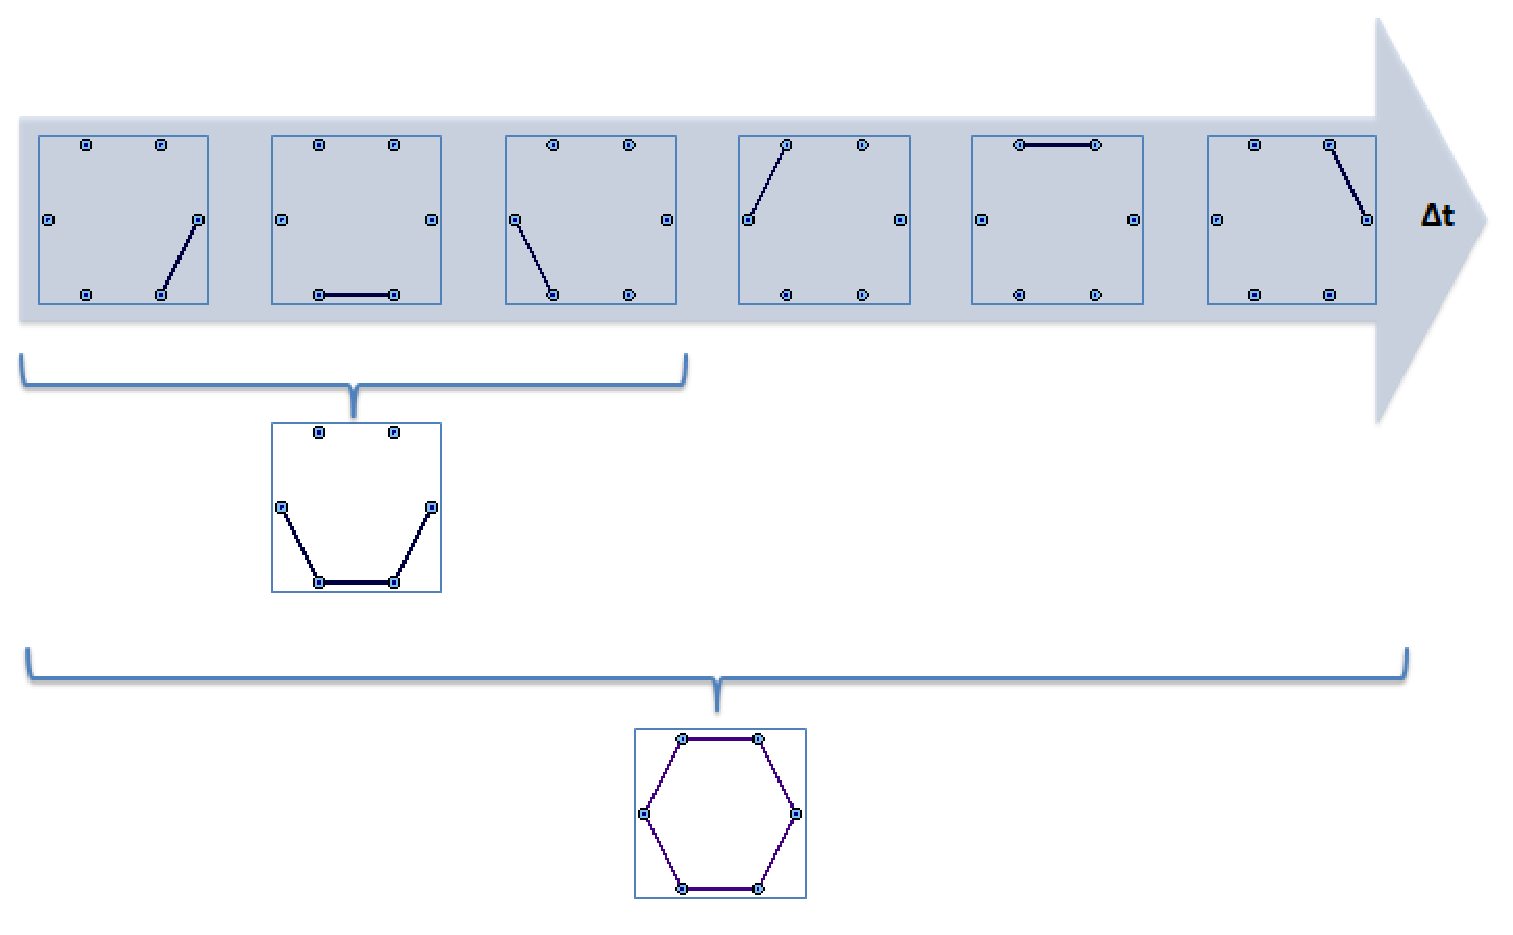
\includegraphics[width=\linewidth]{time_windows}
}

\headerbox{Navigationsalgorithmus}{name=references,column=0,below=Ziel,above=bottom}{
Die Navigation des Roboters erfolgt durch einen drehbaren Ultraschall-Sensor, der seine Umgebung in einem Bereich von 180 Grad in zehn Segmenten abtastet. Daraufhin werden freie Wege und Hindernisse erkannt und eine geeignete Fahrtrichtung zum Ziel errechnet. Der Ablauf ist wie folgt:
\vspace{-.25cm}
\begin{itemize}
\setlength\itemsep{-.25em}
\item[1.] Berechnung der gewünschten Fahrtrichtung anhand der aktuellen GPS-Daten und der Richtung zum Ziel
\item[2.] Abfrage der Sensoren zum Auffinden von Hindernissen
\end{itemize}
\begin{center}
	\vspace{-.25cm}
	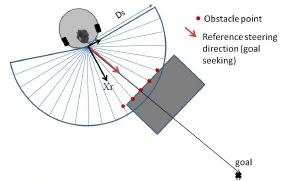
\includegraphics[width=5.75cm]{Bilder/navigation3}
\end{center}
\vspace{-.75cm}
\begin{itemize}
\setlength\itemsep{-.25em}
\item[3.] Einteilung der Segmente in frei und belegt anhand der Sensordaten
\item[4.] Einteilung der freien Segmente in große, mittlere und kleine Lücken
\end{itemize}
\begin{center}
	\vspace{-.25cm}
	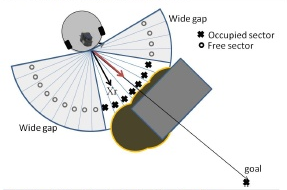
\includegraphics[width=5.75cm]{Bilder/navigation1}
\end{center}
\vspace{-.75cm}
\begin{itemize}
\item[5.] Berechnung der Lenkrichtung anhand der Richtung zum Ziel und den errechneten Lücken, weite Lücken werden bevorzugt.
\end{itemize}
\begin{center}
	\vspace{-.25cm}
	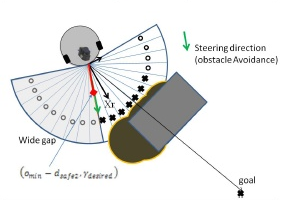
\includegraphics[width=5.75cm]{Bilder/navigation2}
\end{center}
\vspace{-.75cm}
\begin{itemize}
\item[6.] Fahren in die errechnete Lenkrichtung und 
\end{itemize}
\begin{center}
	\vspace{-.25cm}
	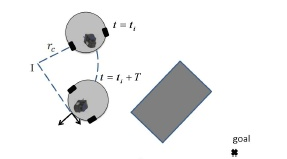
\includegraphics[width=5.75cm]{Bilder/navigation4}
\end{center}
}

%\vspace{1cm}
%\smaller													% Make the whole text smaller
%\vspace{-0.4em} 										% Save some space at the beginning
%\bibliographystyle{plain}							% Use plain style
%\renewcommand{\section}[2]{\vskip 0.05em}		% Omit "References" title
%\begin{thebibliography}{1}							% Simple bibliography with widest label of 1
%\itemsep=-0.01em										% Save space between the separation
%\setlength{\baselineskip}{0.4em}					% Save space with longer lines
%\bibitem{flöte} Flötenroboter Semester \emph{Projektname}, Webseite
%\end{thebibliography}


\headerbox{Aufbau des Roboters}{name=Aufbau,span=2,column=1,row=0}{
\begin{multicols}{2}
Der GPS Roboter besteht aus einem Fernsteuerauto, dessen Fernbedienung durch einen Mini-Computer, einem  Raspberry-Pi, ersetzt wurde. Zusammen mit einem GPS-Modul und Ultraschallsensoren bildet der Raspberry-Pi das Gehirn des Autos. Sensordaten und GPS-Daten dienen dem Raspberry-Pi zur Orientierung. Anhand der Daten errechnet der Raspberry-Pi die gewünschte Lenkrichtung um Hindernissen auszuweichen und das Ziel zu finden.
\begin{center}
\vspace{-.5cm}
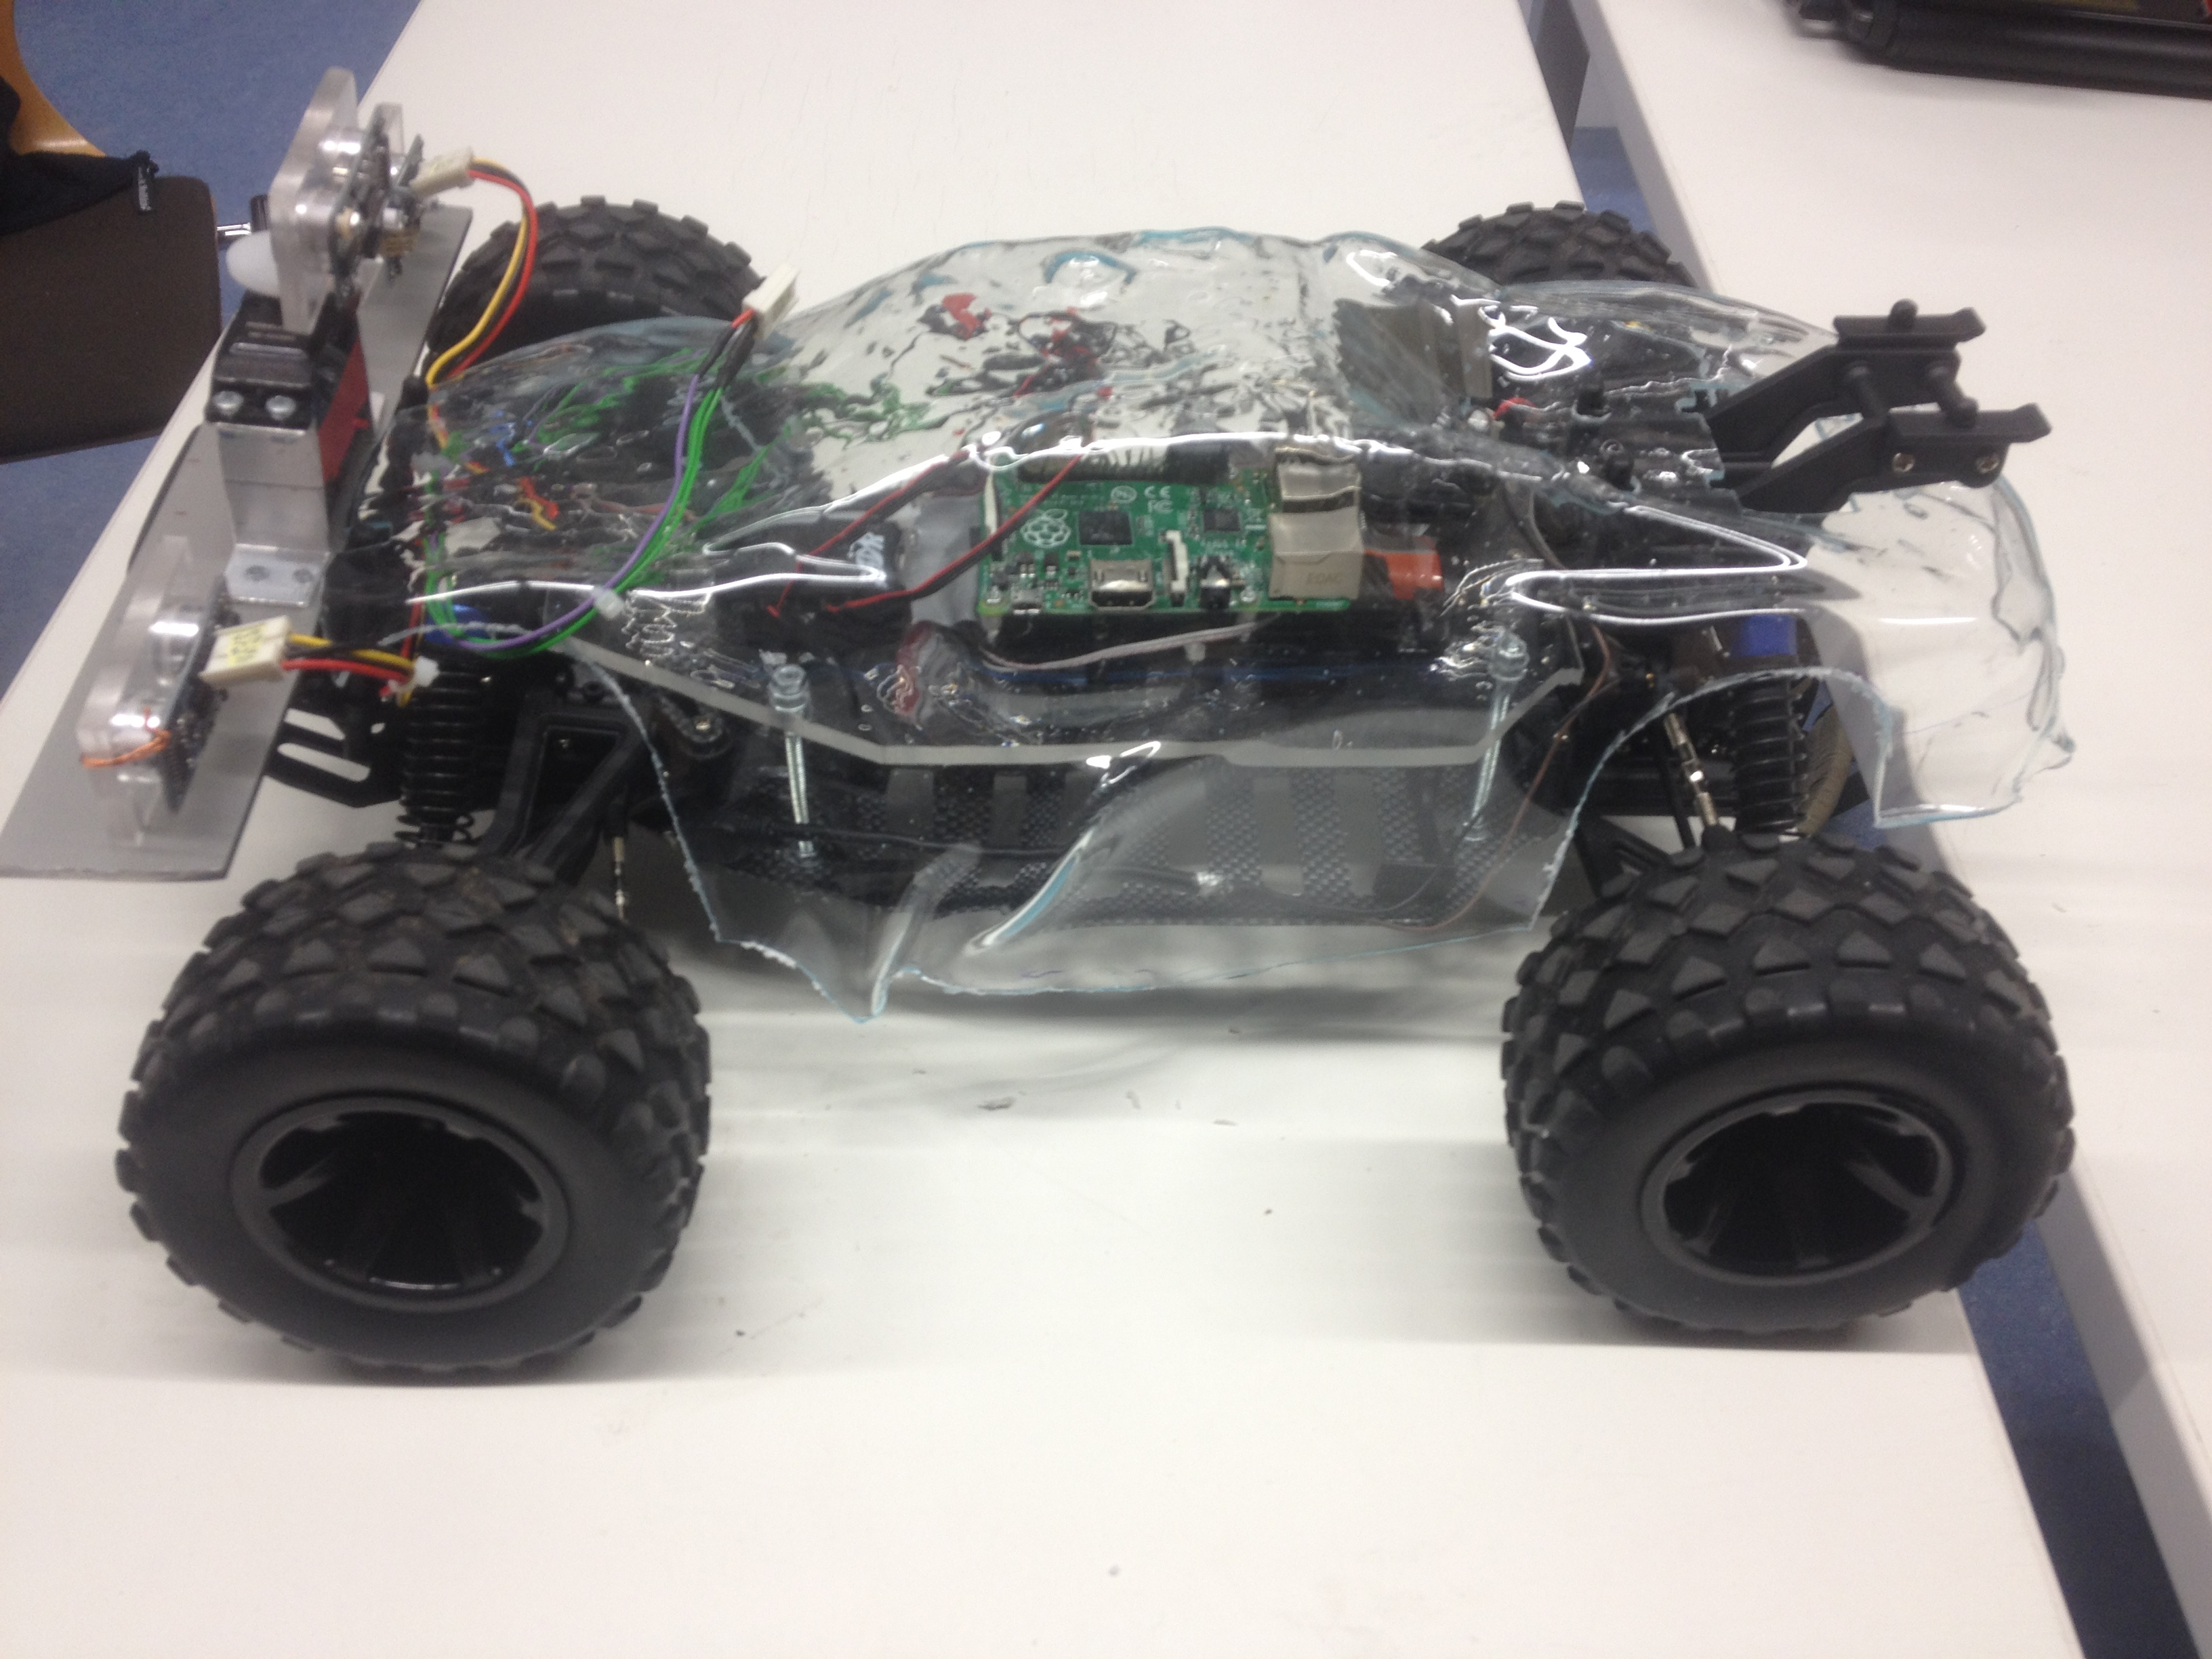
\includegraphics[width=7.5cm]{new_design_II}
\end{center}
\columnbreak
\begin{center}
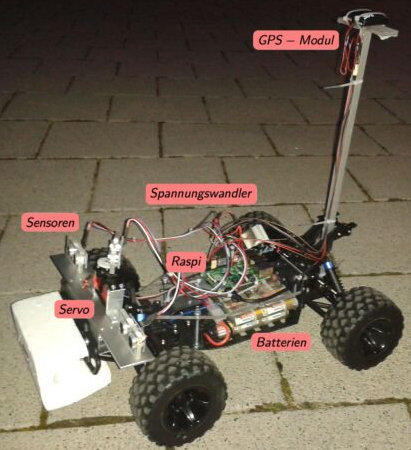
\includegraphics[width=7.5cm]{new_design_IV_new}
%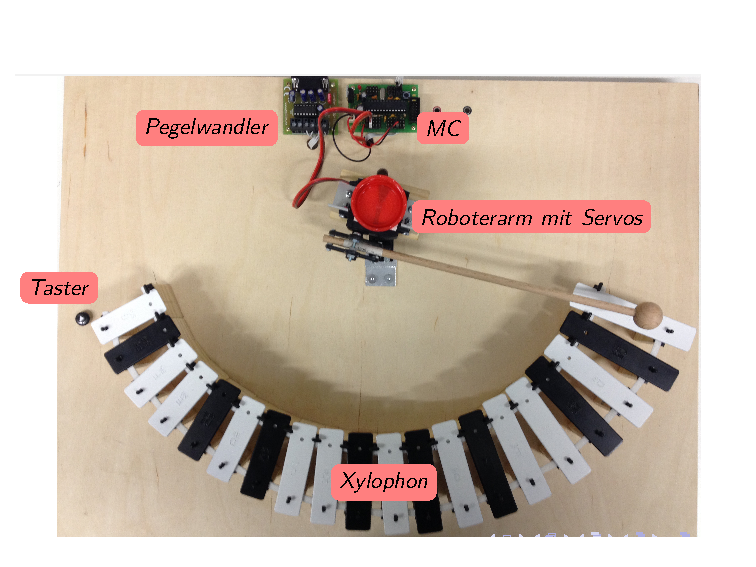
\includegraphics[trim=0cm 0.1cm 0.2cm 0.2cm, clip=true,width=0.65\linewidth]{Aufbau.pdf}
\end{center}
\end{multicols}
}

\headerbox{Steuerung}{name=konzept,span=2,column=1,below=Aufbau}{
Hier wird der schematische Ablauf eines Programmdurchlaufs beschrieben. Zuerst werden Fahrtregler, Sensoren und GPS-Modul initialisiert. Danach startet das Hauptprogramm. Zuerst werden die Sensoren abgefragt um ein direkt voraus liegendes Hindernis zu erkennen. Ist dies nicht der Fall, so startet die Navigationsfunktion. Diese gibt eine Lenkrichtung und einen Motorbefehl (vorwärts/rückwärts) zurück.
Dann übernimmt die Fahrfunktion und führt die errechneten Befehle aus. Danach startet dir Hauptschleife wieder von vorne bis das Ziel erreicht ist.
\begin{center}
	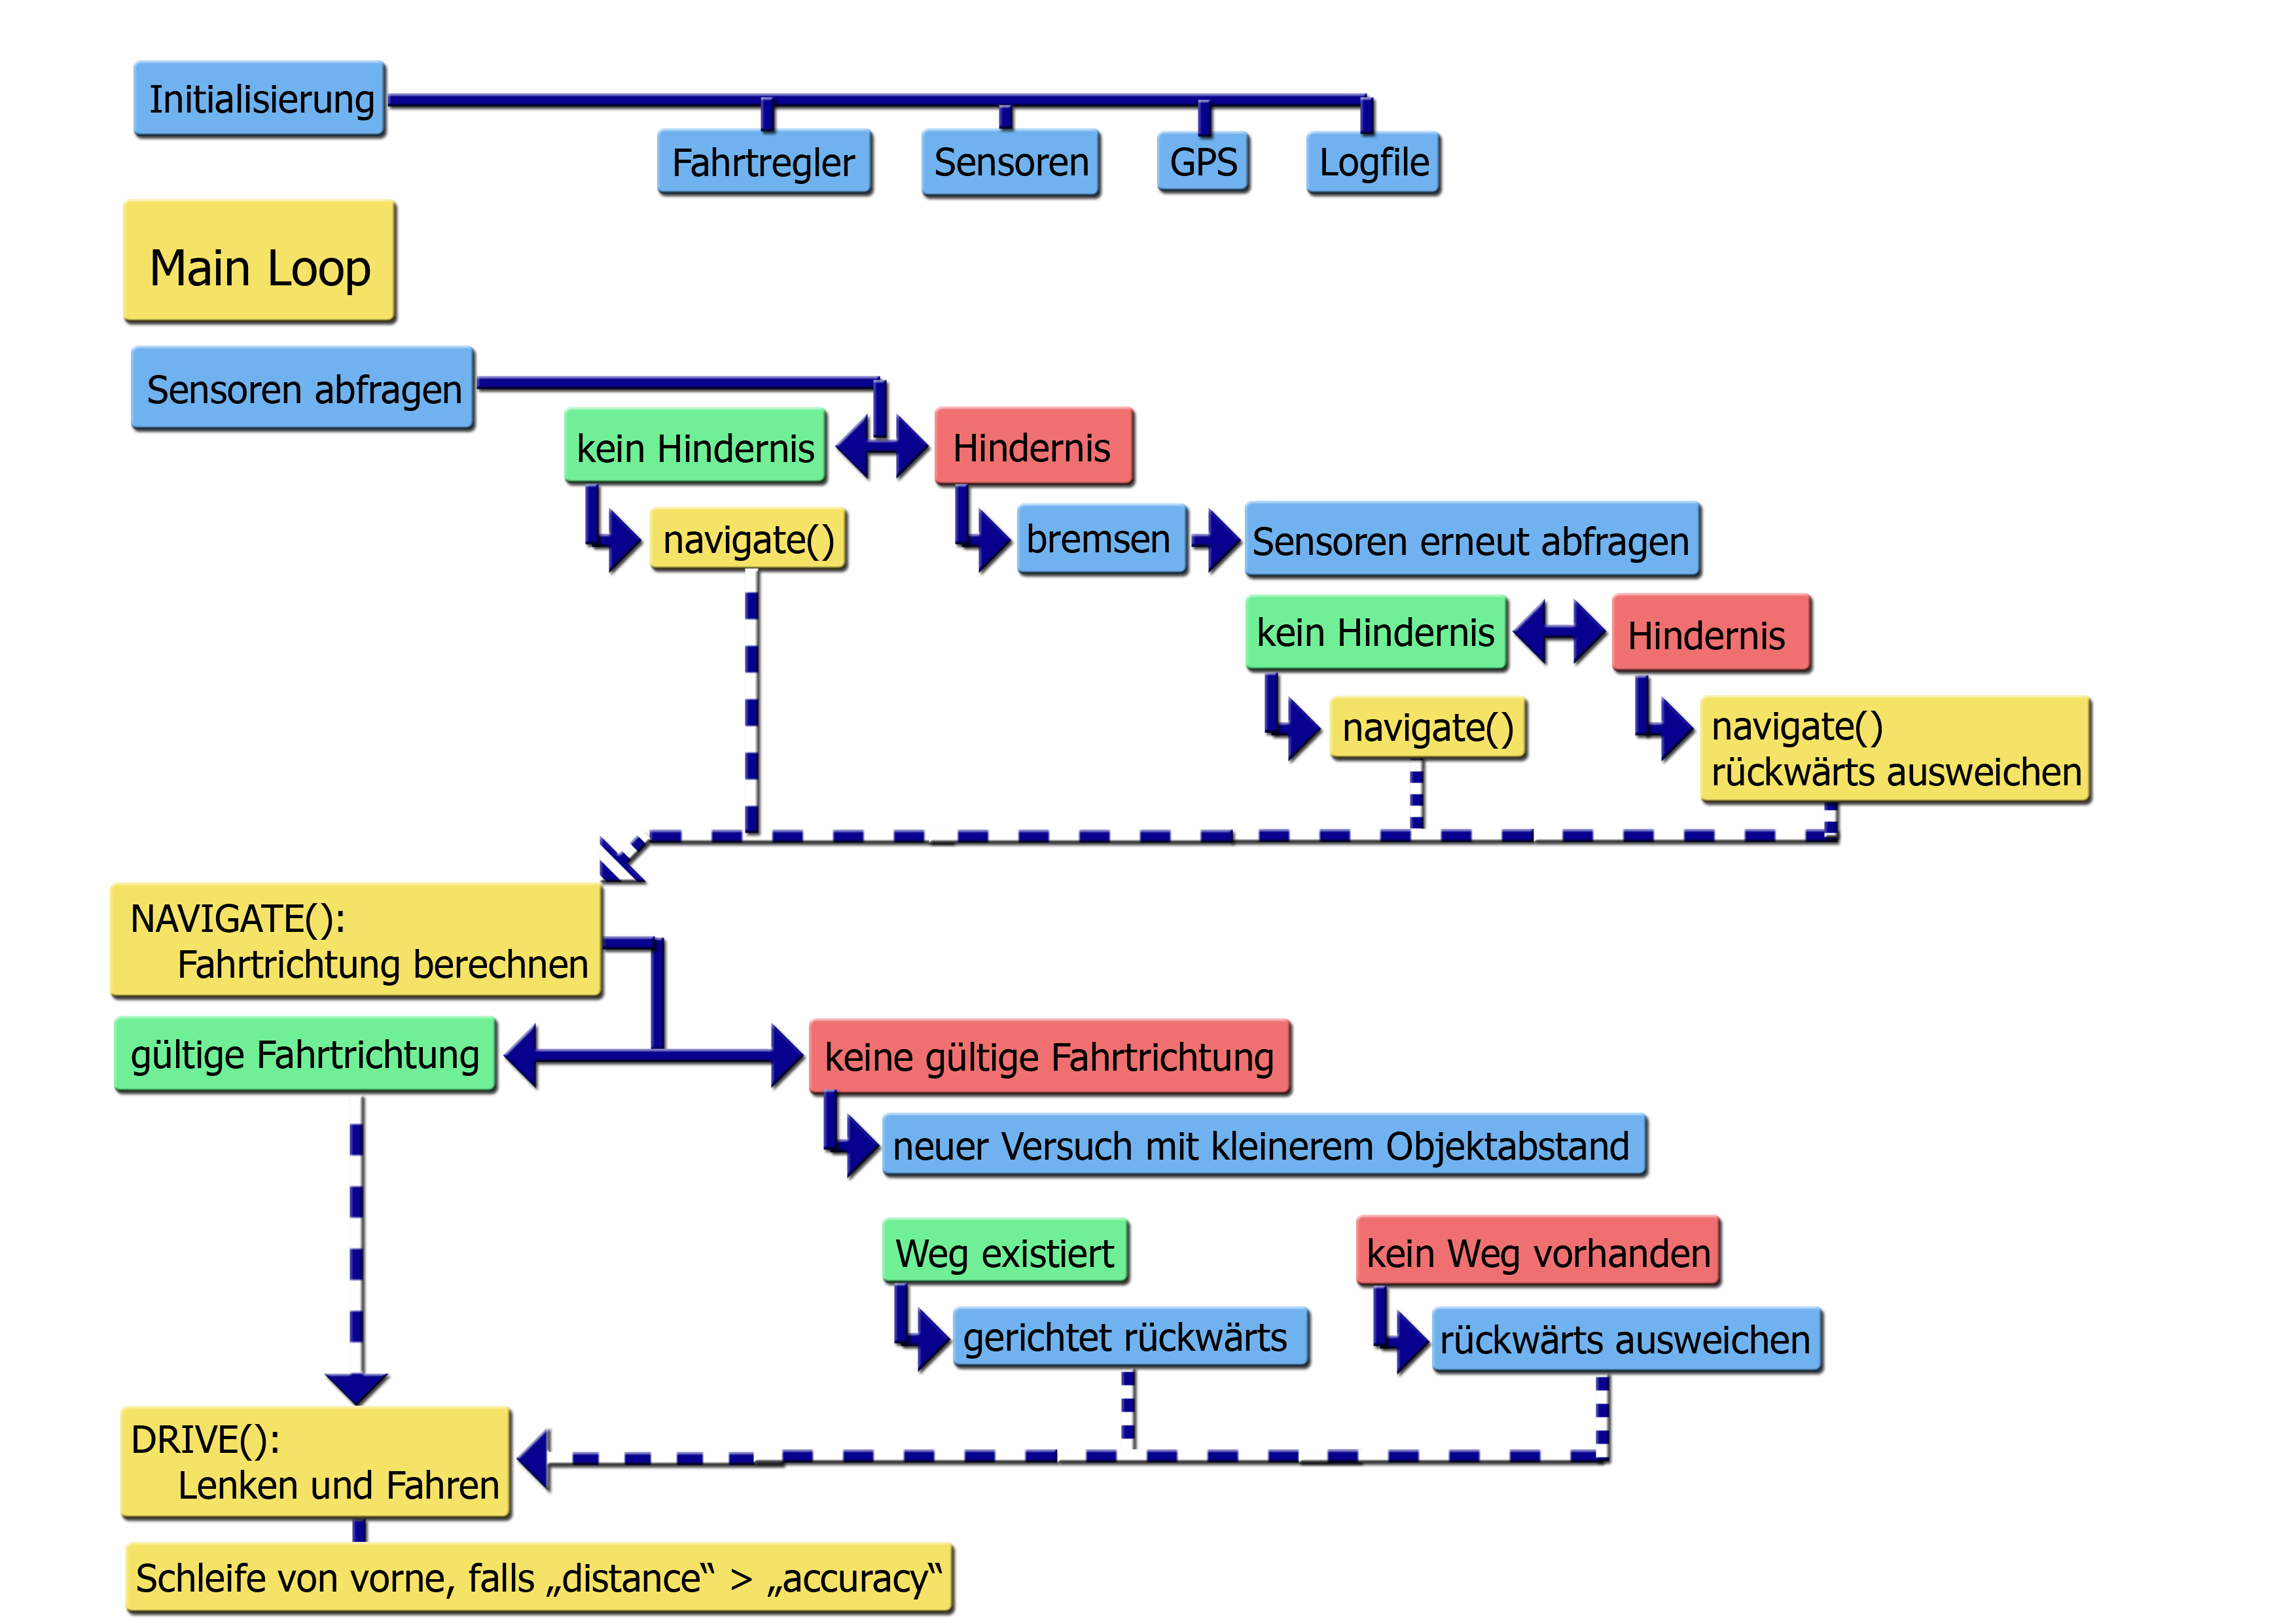
\includegraphics[height=10cm]{Bilder/Flowchart}
\end{center}	
}

\headerbox{Weiterentwicklung}{name=ausblick,column=1,below=konzept}{
%Zur Weiterentwicklung bzw. Verbesserung des Roboters können folgende Punkte umgesetzt werden:
\begin{itemize}
\setlength\itemsep{-.2em}
%\vspace{-0.2cm}
	\item Verfeinerung des Navigationsalgorithmus
%\vspace{-0.65cm}
	\item Verbesserung der Sensoren (z.B. Infrarotsensoren)
%\vspace{-0.2cm}
	\item Einbindung von OpenStreetMaps, Handysteuerung
%\vspace{-0.2cm}
	\item Steuerung des Roboters via Webpage
\end{itemize}
%\includegraphics[angle=-90,width=0.49\linewidth]{team.jpg}
} 

\headerbox{Das Team}{name=team,column=2,below=konzept}{
%\smaller						% Make the whole text smaller
%\vspace{-0.4em}			% Save some space at the beginning
\begin{center}
Maximilian Hartmann\\
9. Semester Physik\\
%\vspace{0.3cm}
Philipp Gernandt\\
8. Semester Physik\\
Tobias Buck\\
9. Semester Physik\\
gps\_robotic@gmx.de
\end{center}
%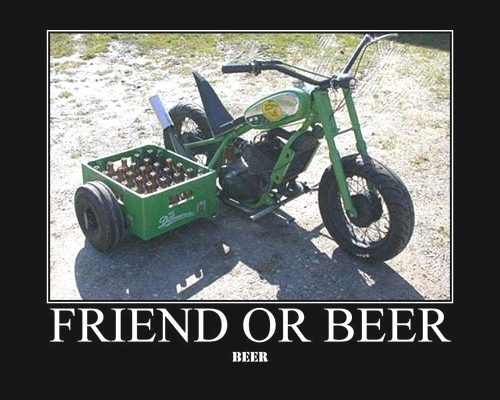
\includegraphics[width=1\linewidth]{23uhr.jpg}
} 

\headerbox{References}{name=ref,span=2,column=1,above=bottom}{
\smaller						% Make the whole text smaller
\begin{multicols}{2}
http://gps-robotic.github.io/Motorization/\\
https://github.com/GPS-Robotic/Motorization\\
http://joanna.iwr.uni-heidelberg.de/rlab/de/home\\
http://cdn.intechopen.com/pdfs-wm/6321.pdf
\end{multicols}
} 

\end{poster}
\end{document}
